%% ============================================================
%%  §1 引言
%%  要证明的一句话：
%%    一层 IR 通吃的假设（源自同构 CPU 时代）在"多框架 × 异构加速器"下失效，
%%    本文把这个失效重述为一个可检验的成本结构问题。
%%  素材：docs/01-outline-v1.md §1（四个必答问题）
%%  建议篇幅：1.5 页
%% ============================================================

\section{引言}
\label{sec:intro}

%% TODO(问题陈述)：不要用"随着深度学习的发展"开头。
%% 直接从算账开始：一个编译器要同时面对 K 个前端与 J 个后端，逐对适配的成本是乘法的。
%% 必须给出具体数字（N 与 M），每一处数字配脚注来源。

%% TODO(为什么一层不够)：引用 §2 的结论——每个系统都固定在某一层，而固定点越低前端越厚、
%% 越高后端越厚（表 1）。所以"选一层"是权衡，不是可以回避的问题。

%% TODO(本文命题)：写成可被推翻的形式。
%% 关键：不要说"MLIR 解决了 N×M"。

%% TODO(贡献三条)：
%% ① 把 N×M 叙事重构为"成本重分配 + 条件性收益"；
%% ② 用 MLIR 自身测试语料量化层间结构（|E| = 76，且是下界）；
%% ③ 给出可代入的成本模型与交叉点 N*，并做 p 的敏感性分析。

%% TODO(不做什么)：不做性能评测、不评判框架优劣、不覆盖全部 LLVM 生态。

%% ---- 图 1：成本模型（立问题） ----
%% 说明：单栏模式下 figure 已是整栏宽，可直接用 \linewidth。
%% 用 PNG 先保证能编译；确认无误后可改用 \includesvg{figures/fig3_cost_model}。
\begin{figure}[t]
  \centering
  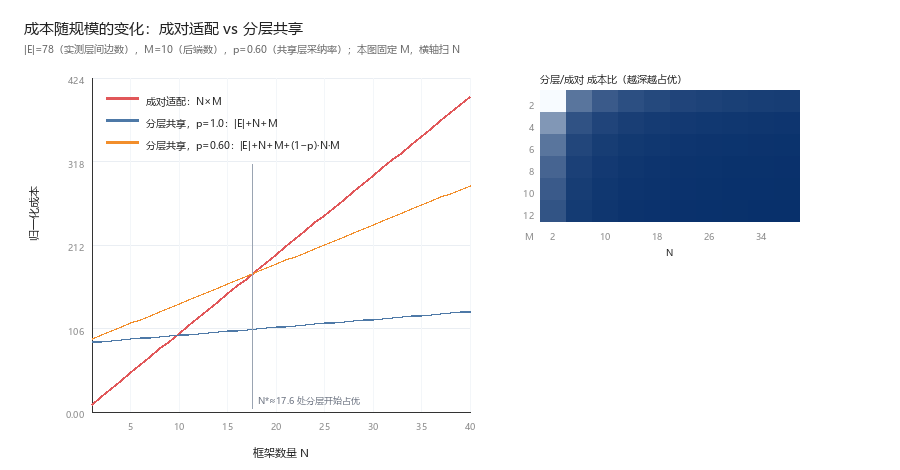
\includegraphics[width=\linewidth]{figures/fig3_cost_model.png}
  \caption{成本随规模的变化。实线为成对适配 $N\cdot M$；虚线为分层共享
  $|E|+N+M+(1-p)\cdot N\cdot M$（$|E|=76$，$M=11$，$p=0.6$）。
  竖虚线为交叉点 $N^\ast\approx15.5$。右图为 $(N,M)$ 平面上的成本比。}
  \Description{左图为三条成本曲线与交叉点，右图为成本比热力图}
  \label{fig:cost}
\end{figure}
